% !Mode:: "TeX:UTF-8"
% !TEX root = ..\thesis.tex
\chapter{研究对象现状与分析}
本文以某汽车电子有限公司的装配车间为研究对象,进行调研。本章将介绍该公司车间的基本情况,并对现有装配线调度情况进行初步分析,指出现有计划安排和调度存在的主要问题,然后针对这些问题,提出合理改进方案。

\section{公司基本情况分析}
该汽车电子有限公司主要产品为车用电子电器开关、控制模块、控制面板等,是美国通用、德国大众、一汽大众、上海大众等国内外40余家汽车主机厂的专业定点配套供应商,配套的代表性车型有奥迪A6(L)、奥迪A4(L)、奥迪Q5、捷达等系列轿车,以及卡车、轻型车、微型车等,产品型号达6000余种。

该公司的订单特点是品种多、批量大、小型产品、工艺成熟,所以采用流水线生产是比较合适的,与其合作较多的客户(主机厂)一般有其专用线,专门负责该主机厂的订单生产。订单从接受到交付的流程如\reff{fig:orderflow}所示,其中虚线框内为装配车间的作业。在没有订单或者订单较少时,为了不让生产线停下来,需要进行工厂内部的计划生产,而订单较多时需要加班作业。
\begin{figure}[h]
\centering
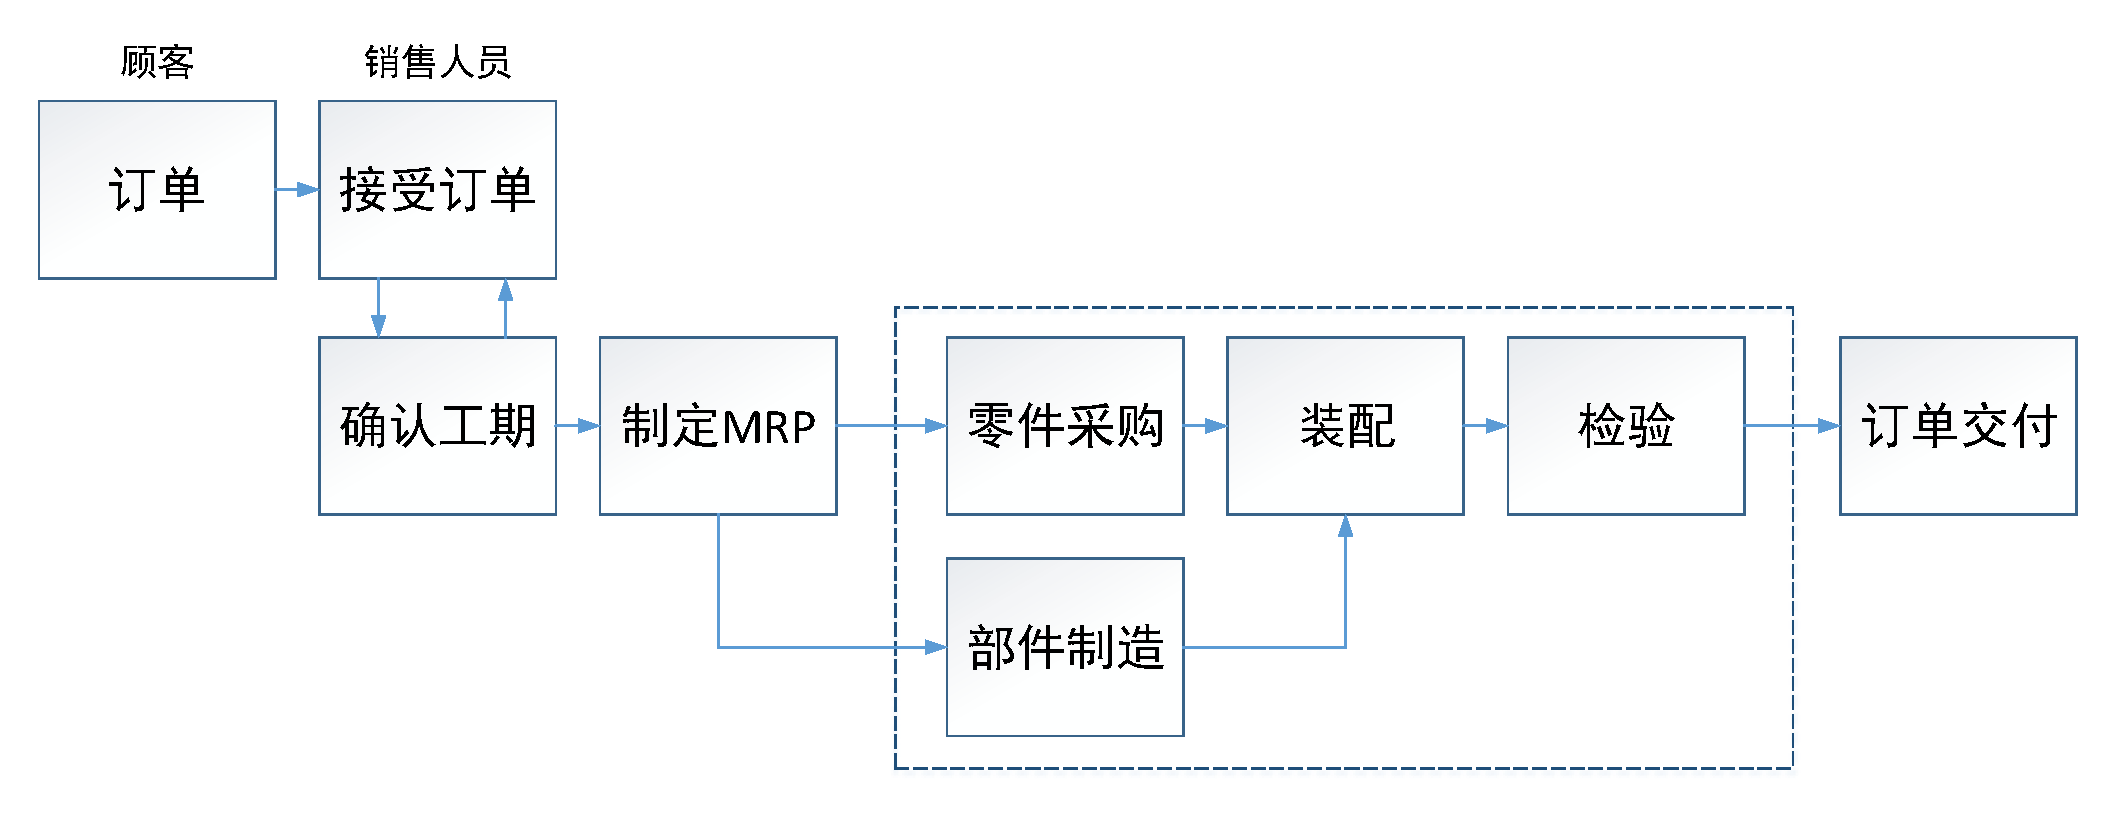
\includegraphics[width = 13cm]{orderflow.pdf}
\caption{现行订单信息流\label{fig:orderflow}}
\end{figure}
\section{装配车间作业信息}
该公司的制造部分为制造一部和制造二部,制造一部主要是负责零部件的生产,不是本课题的主要研究对象;制造二部主要是负责产品总装,共8个车间,均是流水线作业,是本课题的研究对象,其相关信息如\reft{tab:2jobshopinfo}所示。
\begin{table}[htbp]
  \centering
  \caption{制造二部装配车间信息(单位:个)}
    \begin{tabular}{cccccccccc}
    \toprule
    \multicolumn{2}{c}{车间 } & 1车间   & 2车间   & 3车间   & 4车间   & 5车间   & SGM车间 & 通用车间  & 电子车间 \footnote{包括:模块线、插件线及SMT线三个部分,其中,模块线是总装线,共5条装配线,插件线和SMT线是零部件生产线。本次研究的重点是总装线,故电子车间只列出了部分信息。} \\
    \midrule
    \multicolumn{2}{c}{班 组 数 量} & $6$     & $6$     & $6$     & $5$     & $4$     & $4$     & $6$     & $2$ \\
    \multicolumn{2}{c}{流水线数量} & $7$     & $7$     & $7$     & $6$     & $7$     & $6$     & $5$     & $5$ \\
    \multicolumn{2}{c}{PMC分配品种数} & $777$   & $557$   & $186$   & $196$   & $334$   & $29$    & $76$    & $83$ \\
    \bottomrule
    \end{tabular}
  \label{tab:2jobshopinfo}
\end{table}

每个总装车间均有多条生产流水线,为方便管理,每条流水线负责各自对应主机厂的装配生产。当主机厂需要多个品种的产品时,流水线根据订单顺序进行装配作业,即同一主机厂的产品在一条生产线上轮番生产。

\section{多品种装配车间问题分析与解决思路}
当前该公司装配车间采用专线生产的方式,即客户的订单在其专用的流水线上进行装配生产作业,当同一客户有多个订单下达时,按照先到先服务(FCFS)的规则进行装配生产安排,多条产线并行作业互不干扰。

订单或任务到达时,如果有流水生产线空闲可用,则立刻对其根据进行生产准备,然后开始装配生产。若产线在处理订单,那么将该订单安排入其专线队列中,等待前面的批量订单生产完毕再进行生产。现行调度的产线如\reff{fig:3nowschedule}所示,其中订单a -- b 表示主机厂a 的第b 个订单,下同。
\begin{figure}[h]
\caption{$3$条生产线的现行调度\label{fig:3nowschedule}}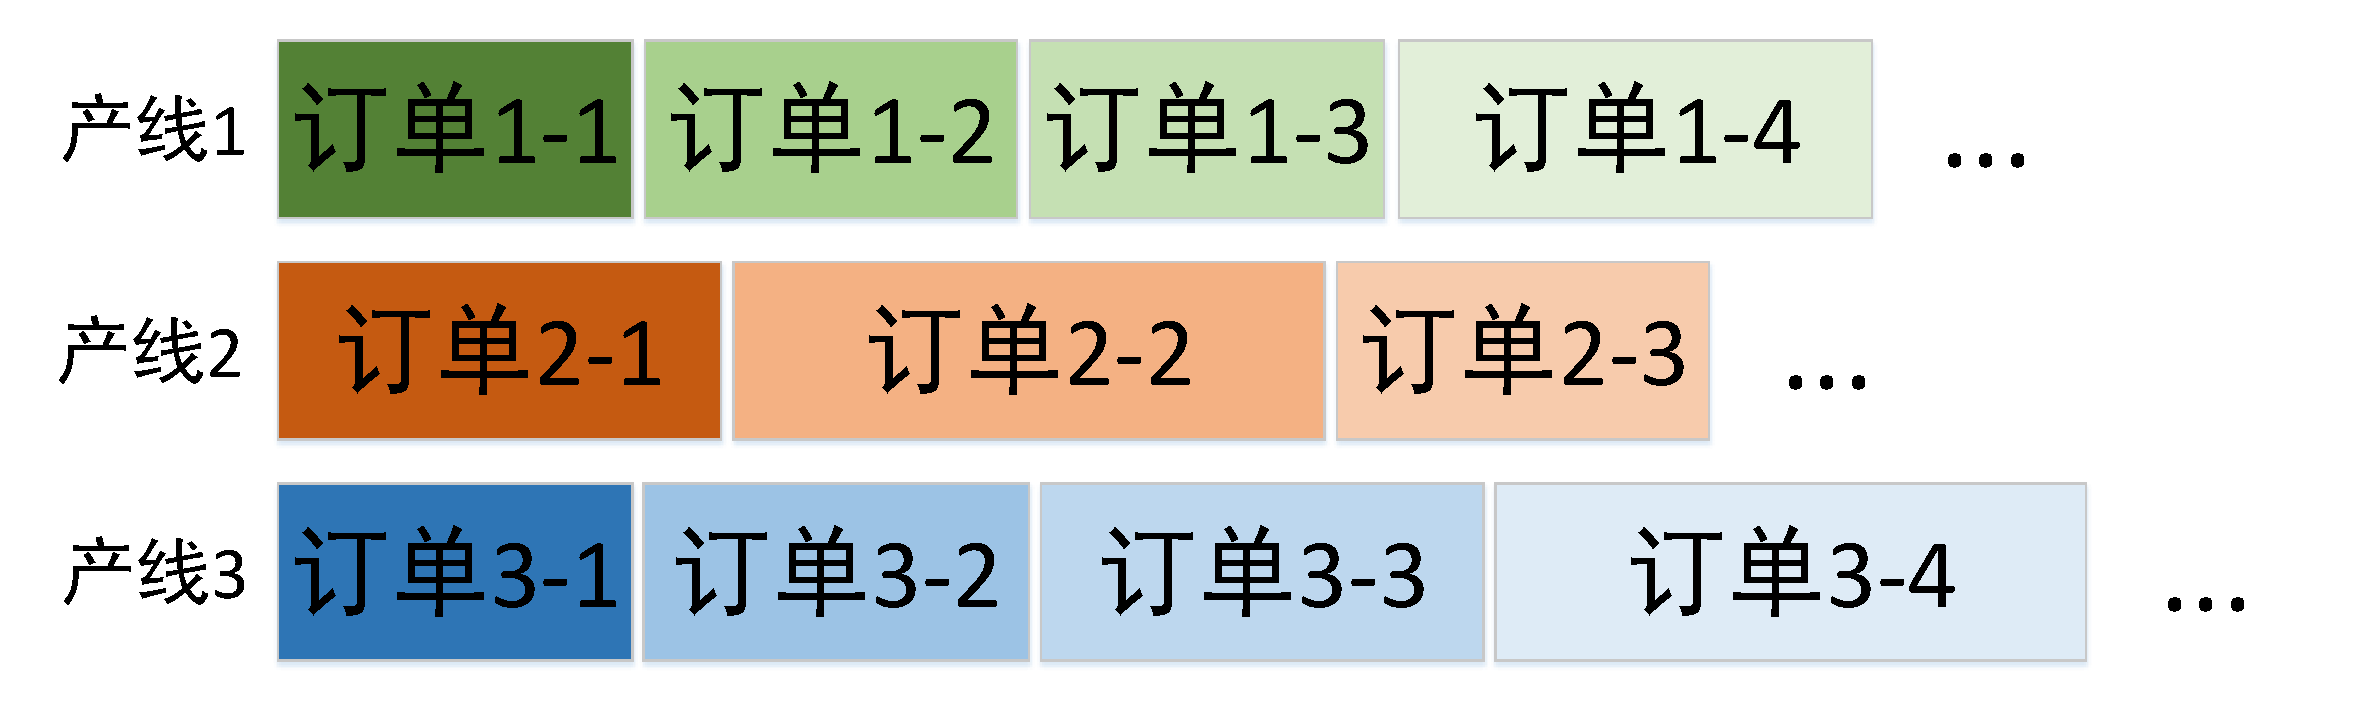
\includegraphics[width = 8cm]{orderschedulenow.pdf}
\end{figure}

现行调度方法逻辑简单,执行力强,客户满意度高,每条装配线可分时生产不同品种的产品,而且按照厂家来安排组织生产,方便了管理。然而其缺陷也是明显的,例如常常会产生有些流水线队列很长而有些流水线空闲无作业的流水线不均衡现象,造成极大浪费。下面进行具体的现有问题分析。

课题研究对象是该汽车电子公司的总装生产线,是典型的流水车间,每条流水线负责一家主机厂的不同品种产品总装流程。装配生产根据订单到达先后进行安排,根据先到先服务(FCFS)规则在相应流水线生成任务队列。

生产线分析包括上述这些差别及其产生的影响或效果,具体描述从订单、装配到交付的流程,并分析现行调度方案的一些指标。

\subsection{现行流程描述}
现行下达订单到交付的流程如\reff{fig:orderflow}所示,销售人员接到客户订单,在确认工期后,将之送达计划部门,制定主生产计划(MRP),随后根据产品特性安排采购与厂内加工。根据任务队列与批量进行产品总装,通过质检包装后,销售人员安排运输送达至客户。
订单到达会立即安排入其对应的主机厂专用产线,当同一主机厂有多个订单同时到达时,则根据最早交货期(EDD)规则进行安排。

本课题的研究对象是流程中的总装调度安排,即为虚线框内的部分,其重点在订单的装配生产安排上,故要进行先行调度方案分析,发现问题。
\subsection{现行调度方案}
如前所述,先行调度方案十分简单,容易操作,由于客户专有各自的装配流水线,所以流水线上的生产安排只需按照客户下达订单的顺序即可,不同车间、不同流水线之间没有相互的联系。由于各流水线上没有专门的工装夹具,一般都是根据订单的内容,在其到达时快速布置流水线的各个工位,所以同一主机厂的连续订单生产时,需要考虑切换准备时间。

现行调度方案逻辑简单,执行力强,每条装配线可分时生产不同品种的产品,而且按照厂家来安排组织生产,方便了管理。
\subsection{主要问题}
现行调度方案存在一些问题,是本课题所研究的改进空间,例如多条装配线负荷不均衡,有的任务过重,有的任务不足,负荷不均衡,一条装配线上装配的产品工艺相似性较低,导致换线时间增加,产生更长的等待。

根据现行调度情况进行问题分析,可以归纳其主要存在问题如下:
\renewcommand{\labelenumi}{(\theenumi)}
\begin{asparaenum}
\item 产线利用率低
\suspend{asparaenum}

产线利用率低主要体现在存在大量换线时间,一方面由于产线等待队列由FCFS 规则产生,同时到达的订单也只是根据EDD 规则安排,没有考虑品种装配流程间的相似性。当这种差异很大时,必然会增加换线时间,进而增加了任务间的等待。另一方面,由于产线的专用性,当有多条产线都能处理某个任务时,该任务只能在订单来自的主机厂专线上生产,闲置了可用线的生产能力。
\resume{asparaenum}
\item 生产不均衡
\suspend{asparaenum}

这里的生产均衡和混流生产中的均衡生产稍有差别,此处的不均衡现象更为宏观。来自不同主机厂的任务在不同产线上进行处理,这样一来,订单较多、较频繁的主机厂产线总是会处于繁忙状态,而订单较少的产线则呈现为停线等待居多。这种不均衡现象直接导致产能的巨大浪费,同时也间接导致了换线时间增加,因为不均衡的生产业表面订单较为集中。突破专线限制可以解决宏观不均衡问题,虽然细分到单条线上的混流生产可以近一步均衡化生产,但其需要较高的管理投入,可以考虑折衷。
\resume{asparaenum}
\item 产线冗余度高
\suspend{asparaenum}

前面几大问题已经涉及到了一些浪费现象,除了这些之外,该厂制造二部共有8个装配车间,每个装配车间有7--8条总装流水线,然而由于流水线是按主机厂进行分配,存在较高的冗余度,前面提到的产线间设备类似属于其中之一。产线的冗余还包括作业及管理人员,辅助设置,场地空间,相关能源等。
\resume{asparaenum}
\item 工期可控性低
\suspend{asparaenum}

工期的可控性低主要体现在应变插单的问题上,现行调度采用的是不可中断的流水作业,各流水线只能按其队列顺序进行装配作业,由于这样安排没有顾及工期的先后即订单的具体情况,导致大部分订单都需要延期交货,也存在较多订单的过早完工,增加了库存。此外,虽然插单可以较为合理安排订单加工顺序,而然会带来额外的切换时间,需要权衡考虑。
\resume{asparaenum}
\item 工艺及设备和生产需求不匹配
\end{asparaenum}

各流水线需要有多品种加工的能力,故线上需要有相应加工工艺的设备,而时常不同主机厂所需产品可能有很高的相似性,这使得同样的设备需要在多条流水线上设置,尤其对于加工时间较短、处理批量较少的作业,过多的设备徒增成本与闲置。另一方面,加工时间长、处理批量大的作业,较少的设备不利于生产效率,导致在制品增多。

\subsection{改进设计}
对问题的产生原因进行分析,这为改进调度方案明确了方向。
为制定合理调度方案,改善装配流水线现状,首先需要确定改进目标,进而根据目标的可行性,建立数学模型,权衡投入和效益,建立适合本课题研究对象的多品种多装配线轮番装配生产调度模型。

目前的生产现状的主要问题是各主机厂有其专用流水线,使得订单的调度安排为较为单一,受到一些限制,不能很合理地利用流水线的生产能力,所以首要的改进是突破专用线的生产界限。如此一来,生产线可以加工多家主机厂的订单,形成所谓的混线生产,是较混流生产为宏观的均衡化生产,如\reff{fig:orderschedule}所示
。与混流生产不同的是,混流生产的最小研究单位是订单中的作业,而混线生产的最小研究单位是订单本身,即一定批量的作业。混线生产的策略是将不同订单的作业按一定比例进行生产,一般是在单一流水线上进行研究的,可使生产均衡化,但这一策略需要分析不同作业的相似程度,相差太大的作业若混流生产则会导致过多的切换准备时间,而且这个策略需要较高的管理水平。混线生产考虑的是多流水线之间的订单调度安排,使流水线的利用更为充分。

突破主机厂专用线限制后,出现了多品种多装配线的混流生产调度的问题,可以表述为,不同主机厂下达的不同订单到装配流水线车间,所有的订单可以在任意流水线上进行装配生产,需要建立合适的调度方案以合理利用各流水线的生产能力以及其他生产装配目标。

\begin{figure}[h]
\centering
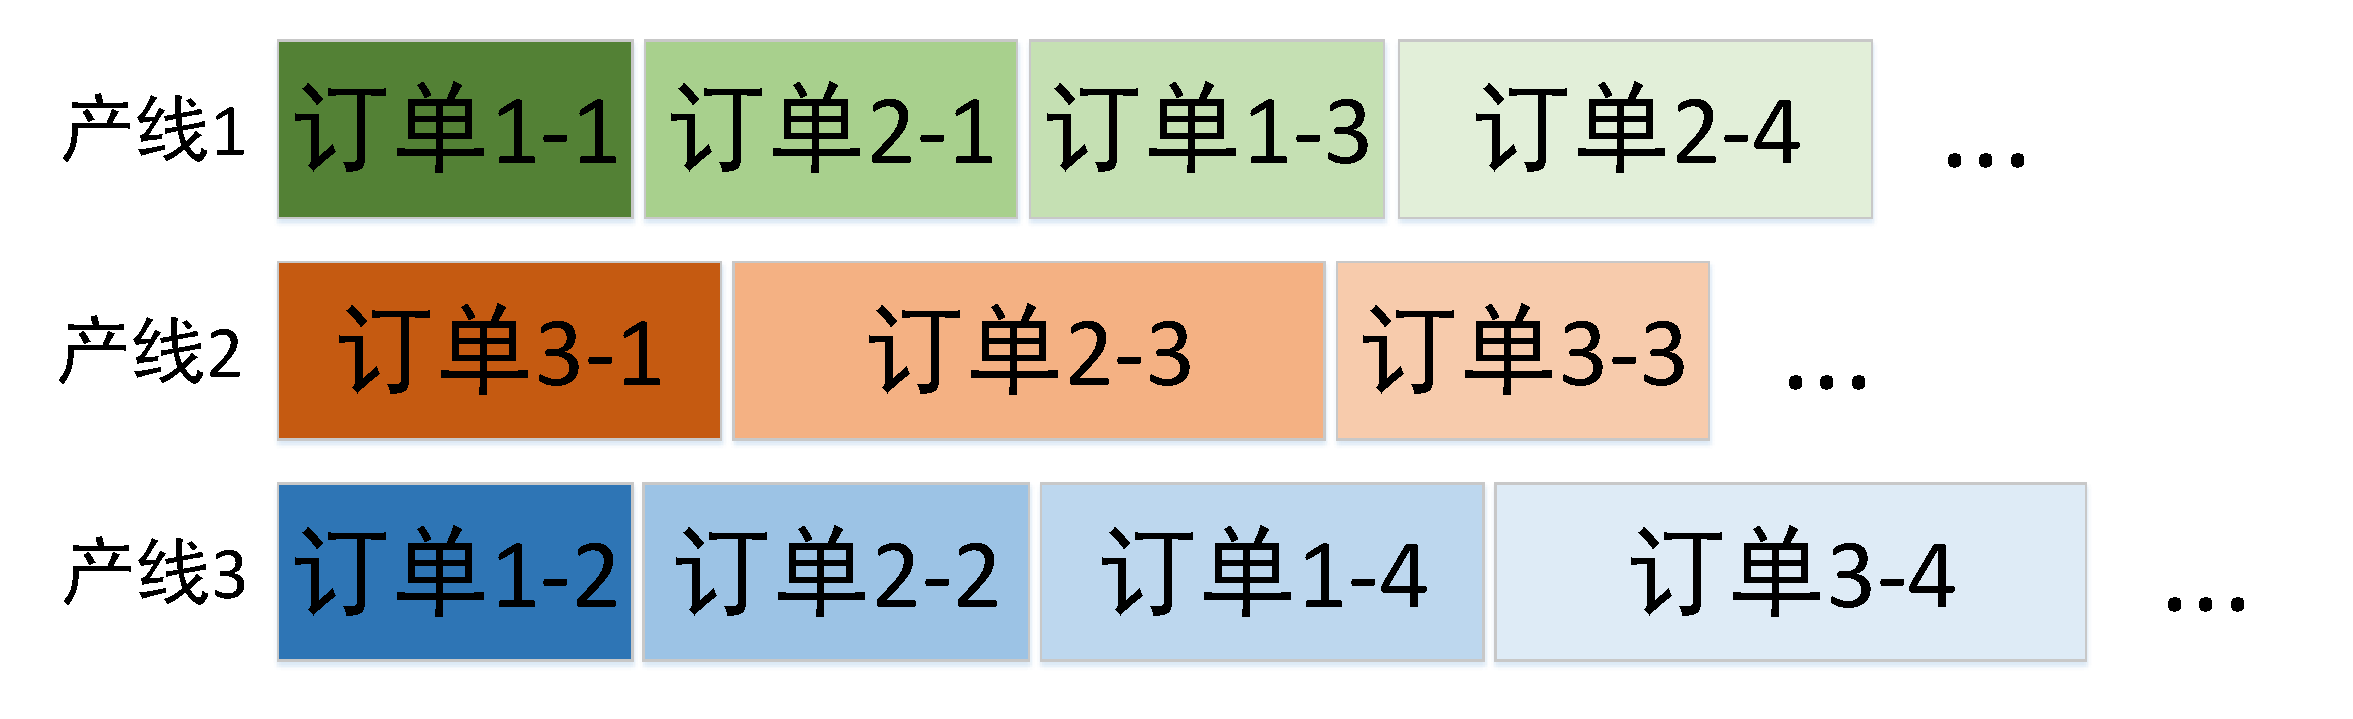
\includegraphics[width = 8cm]{oredrschedule.pdf}
\caption{$3$条产线的混线装配生产示意\label{fig:orderschedule}}
\end{figure}

\section{小结}
本章简单介绍了该汽车电子有限公司的装配车间生产现状及其问题,并提出了解决方案,以此引导出了多品种多装配线的混流生产调度问题,需要建立合适的调度方案。调度方案的建立即该问题的求解,需要通过问题分析与建模,并设计相应的算法来求解。